\chapter{Methodology}  

\section{Bayesian Model}

In this section, we delve into a comprehensive understanding of the Bayesian model's implementation. To begin, we explore the fundamental elements that serve as the foundation for our analysis: the events matrix and the Blood Oxygen Level Dependent (BOLD) data. These are the core ingredients that provide insights into brain activation patterns during an fMRI experiment. Furthermore, we delve into the practical application of image masking. And finally, we will unravel the implementation of the Bayesian model.

\subsection{Design Matrix ($X$)}

To convert events matrix from an fMRI experiment into a design matrix using Nilearn, one should first import the necessary libraries, including Nilearn, and load the events data into a DataFrame. With Nilearn's  \texttt{make\_first\_level\_design\_matrix} function, a design matrix can be created by specifying event onsets, durations, the repetition time (TR) of the fMRI data, and other parameters like drift modeling and the hemodynamic response function (HRF) model. This design matrix reflects the temporal relationship between events and the fMRI data. Then, the design matrix can be visualized to inspect how the events are modeled in relation to the fMRI data. Finally, this design matrix can serve as a crucial regressor in various fMRI analyses, enabling researchers to investigate neural activity patterns, perform statistical tests, and gain valuable insights from the fMRI experiment. Figure \ref{fig:c3_DesignMatrix} presents an example of a design matrix generated for an fMRI experiment.

\begin{figure}[htbp!]
\centering
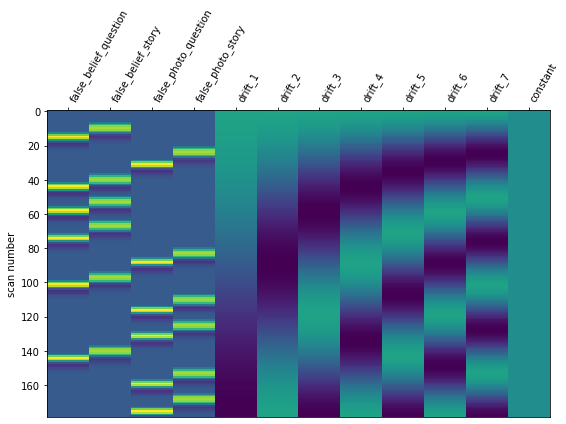
\includegraphics[width=0.7\textwidth]{images/DesignMatrix.png}
\caption{Design Matrix Example}
\label{fig:c3_DesignMatrix}
\end{figure}

\subsection{Time Series ($\bm{y}$)}

Converting the 4D BOLD data from an fMRI experiment into voxel time series is a crucial step in neuroimaging analysis. To achieve this, one must first load the 4D data, which represents a sequence of 3D brain scans collected over time. By specifying the coordinates of a voxel within the 4D dataset, researchers can extract the time series data, typically using neuroimaging libraries like Nilearn or nibabel in Python. This extracted time series provides a dynamic record of neural activity for the chosen voxel. Figure \ref{fig:c3_TimeSeries} presents an example of a time series for a certain voxel of an fMRI experiment.

\begin{figure}[htbp!]
\centering
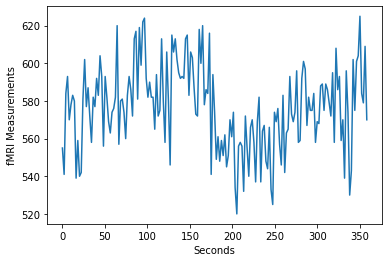
\includegraphics[width=0.7\textwidth]{images/TimeSeries.png}
\caption{Voxel Time Series Example}
\label{fig:c3_TimeSeries}
\end{figure}

\subsection{Image Masking}

Masking fMRI data using Nilearn is a crucial preprocessing step in neuroimaging analysis. To begin, the fMRI data is loaded, and a region of interest (ROI) is defined using a mask image that specifies the brain areas to be analyzed. Nilearn provides a helpful function, \texttt{nilearn.masking.compute\_epi\_mask}, to create a mask automatically based on intensity thresholds from the fMRI data. This mask is then applied to the fMRI data using \texttt{nilearn.masking.apply\_mask}, resulting in a masked dataset. The masked data retains only the information within the specified ROI, allowing for focused and more precise analyses of brain activity in the defined region. This process is instrumental in narrowing down the scope of the analysis to specific brain areas or volumes of interest, facilitating more accurate and targeted neuroimaging investigations. Figure \ref{fig:c3_Mask} presents an example of the results of a masking process in an fMRI data.

\begin{figure}[htbp!]
\centering
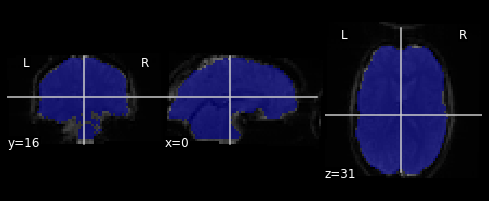
\includegraphics[width=0.7\textwidth]{images/Mask.png}
\caption{Masking Results Example}
\label{fig:c3_Mask}
\end{figure}

\subsection{Implementation}

In the implementation osf the model, frequency probability played a pivotal role in understanding the activation patterns within fMRI data. For each experimental session, a design matrix $X$ was meticulously crafted to capture the dynamics of stimuli presentation, while the time series $\bm{y}$ was acquired for every voxel in the image. The crux of this approach lay in the per-voxel analysis, where 1000 samples of the regression coefficients $\bm{\beta}$ were stochastically generated. These samples were drawn from the conditional posterior distribution in Equation \ref{eq:conditionalPosterior}, a critical component of the model. Subsequently, for each specific stimulus, an essential insight was gained through the calculation of the probability that a particular voxel's coefficient $\bm{\beta}_i$ exceeded zero, indicating the activation of that voxel in response to the given stimulus $i$. This comprehensive analysis, driven by frequency probability, allowed for a nuanced exploration of voxel-specific responses to distinct stimuli, unraveling the intricate dynamics of neural activity within the fMRI dataset.

\section{Adaptive Smoothing and Thresholding (AST) Algorithm}

\section{Adaptive Smoothing Algorithm}

Given probabilistic mapping (PM) $\bm{x} \sim TN(\mu,\sigma^2,0,1)$, we estimate $\mu$ and $\sigma$ by maximizing the following log-likelihood function, see Appendix %\ref{AppendixB} for derivation.
\begin{equation} \label{eq:tn_llf}
l(\bm{x};\mu,\sigma^2) = -n \log \left( \Phi(1;\mu,\sigma^2) - \Phi(0;\mu,\sigma^2) \right)-\frac{n}{2} \log \left( 2\pi \sigma^2 \right) - \frac{\sum_{i=1}^n (x_i-\mu)^2}{2\sigma^2}
\end{equation}

Starting with $\bm{x} \sim TN(\mu,\sigma^2,0,1)$ obtained as explained in Section $3.2$, we propose the algorithm:

\begin{enumerate}
\item \textit{Initial Setup.} Assume that all the voxels are inactive, in other terms, $\zeta_i \equiv 0 \; \forall i$, where $\zeta_i$ is the activation status for the $i$th voxel. Set $\zeta_i^{(0)} \equiv \zeta_i $, $\bm{x}^{(0)} = \bm{x} $, and $n_0 = n$, where $n_k$ denotes the number of voxels for which $\zeta_i^{(k)} = 0$.
\item \textit{Iterative Steps.} For $k=1,2,\dots,$ iterate as follows:
\begin{enumerate}
\item Maximize Equation \ref{eq:tn_llf} given $\bm{x}^{(k-1)}$ to obtain $\mu^{(k)}$ and $\sigma^{(k)}$. Smooth $\bm{x}^{(k-1)}$ with $\mu^{(k)}$ and $\sigma^{(k)}$ to get $\bm{x}^{(k)}$.
\item Get $a_n=\left[n\psi(b_n)\right]^{-1}$ and $b_n=\Psi^{-1}(1-\frac{1}{n})$ to obtain: $$\eta_k = a_{n_{k-1}}i_{\alpha} + b_{n_{k-1}}$$
where $i_{\alpha}$ is the upper-tail $\alpha$-values for the Gumbel distribution. Now, set $\zeta_i^{(k)} = 1$ if $\zeta_i^{(k-1)} = 0$ and the $i$th coordinate of $\bm{x}^{(k)}$ exceeds $\eta_k$. Let $n_k=\sum_{i=1}^n \zeta_i^{(k)}$.
\end{enumerate}
\item \textit{Termination.} ...
\end{enumerate}